\subsection{IDE介绍}
\begin{frame}{集成开发环境-IDE}
    集成开发环境(Integrated Development Environment, IDE): 

    \tiny{用于提供程序开发环境的应用程序,一般包括代码编辑器、编译器、调试器和图形用户界面等工具。
    集成了代码编写功能、分析功能、编译功能、调试功能等一体化的开发软件服务套件。
    所有具备这一特性的软件都可以叫集成开发环境。
    }

    \normalsize
    \begin{columns}
        \column{0.5\textwidth}

        流行的 Python IDE:

        \begin{myoutline}
            \1 \textcolor{blue}{PyCharm} (√)
            \1 \textcolor{blue}{VS Code}
            \1 \textcolor{pink}{Jupyter Lab} (√)
            \1 \textcolor{pink}{Spyder}

            \tiny{\1 IDLE, Sublime, Vim, Emacs\dots}
        \end{myoutline}

        \column{0.5\textwidth}
        
        \begin{figure}
            \centering
            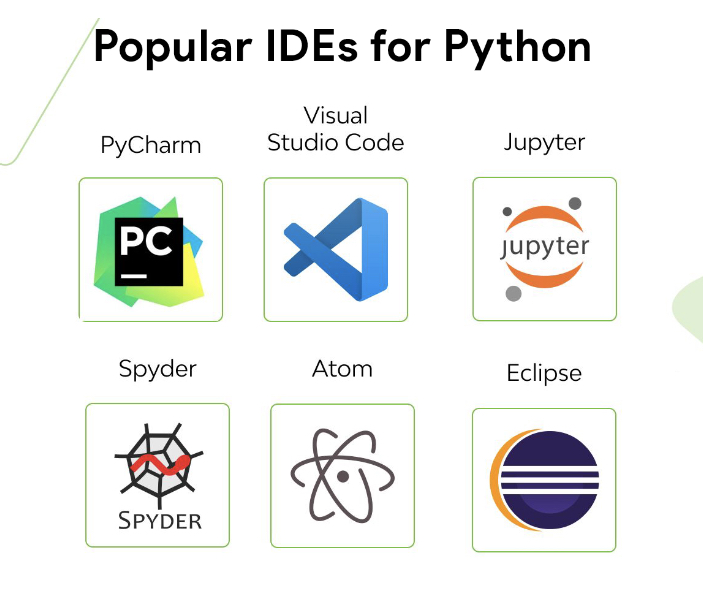
\includegraphics[width=0.7\linewidth]{Images/IDEs.jpg}
        \end{figure}
    \end{columns}

    \footnotenoindex{https://gknxt.com/python/whatisanide.php}
\end{frame}

% \1 PyCharm (工程, 业界)
% \1 VS Code (全能, 小巧)
% \1 Jupyter Lab (数据分析, 机器学习)
% \1 Spyder (数据分析, 机器学习)

% 接下来, 我们就从Python 的工作环境配置开始
% 首先, 我们先来学习一下什么是 IDE

% 以Pycharm,Jupyterlab,VScode
% IDLE, Sublime
% 区别在缩小,概念在弱化
% 会在以后的不同部分中融入进去